\documentclass[a4paper,10pt]{article}

\usepackage{palatino}
\usepackage{mathpazo}           % optional [sc] fuer real small caps
\usepackage[left=3cm,top=3cm,right=3cm,bottom=2cm,nohead,nofoot]{geometry}

\usepackage{graphicx}

\newcommand{\key}[1]{{{\texttt{\textbf{#1}}}}} % this does nasty things to underscores
\newcommand{\sex}[1]{{{\textbf{#1}}}} % \sec already defined

\newcommand{\crawl}{\textsc{Crawl}}
\newcommand{\dungeon}{\textsc{Dungeon}}

\newcommand{\spacecolumn}{\begin{minipage}[t]{2cm}\phantom{xxxx}\end{minipage}}
\newcommand{\para}{\vspace{1.5ex}}
\setlength{\parindent}{0em}

\newcommand{\mc}[1]{\multicolumn{2}{l}{#1}}

\newcounter{abccounter}
\newenvironment{abcliste}{\begin{list}{(\alph{abccounter})}
                      {\usecounter{abccounter}
                       \setlength{\topsep}{0ex}
                       \setlength{\partopsep}{0ex}
                       \setlength{\listparindent}{0ex}
                       \setlength{\itemsep}{0ex}
                       \setlength{\parsep}{0ex}
                       \setlength{\leftmargin}{2em}
                       \setlength{\labelwidth}{2em}
                       \setlength{\parskip}{0ex}
                      }
                      }{\end{list}}

\pagestyle{empty}

\begin{document}

\begin{center}\textbf{\LARGE
\dungeon\ \crawl: Very short introduction}
\end{center}

Crawl is a large and very random game of subterranean exploration in a fantasy 
world of magic and frequent violence. Your quest is to travel into the depths 
of the Dungeon (which is different each time you play) and retrieve the Orb of 
Zot. 

\para

Crawl is a game of the 'roguelike' type, one of the descendants of Rogue. Its 
graphics are simple but highly informative, designed to be understood at a 
glance, and control is exercised largely through one-keystroke commands. 

\para\para

\sex{Starting Out} \para

After starting the program you will be greeted with a message asking for your 
name. Don't spend too much time over this, as your first character will 
\emph{not} last very long (sorry, but it's true). 

\para

Next you are given menus of species and character classes from which to 
choose. A dwarf, orc, ogre, or troll Fighter is a good bet. Elves are quite 
fragile, humans are pretty average at everything, and the weirder species are 
mostly too tricky for beginning players. Finally, you may be given a choice of 
weapons. I suggest an axe (axes are fun). 

\para

\begin{minipage}{10cm}
Now you are in the game. The game screen has three parts: \\
The \textbf{Map} takes up the upper left part of the screen. In its very 
centre is the \key{@} sign which represents You. The coloured parts of the map
is the area you can see, while places that you have visited before but cannot
currently see are shown in grey. \\
The \textbf{Message box} is the large part of the screen below the map. It 
describes all events as they happen. \\
The \textbf{Stats area} contains information about your character. 
\end{minipage}
\begin{minipage}{1cm}
\phantom{xx}
\end{minipage}
\begin{minipage}{4cm}
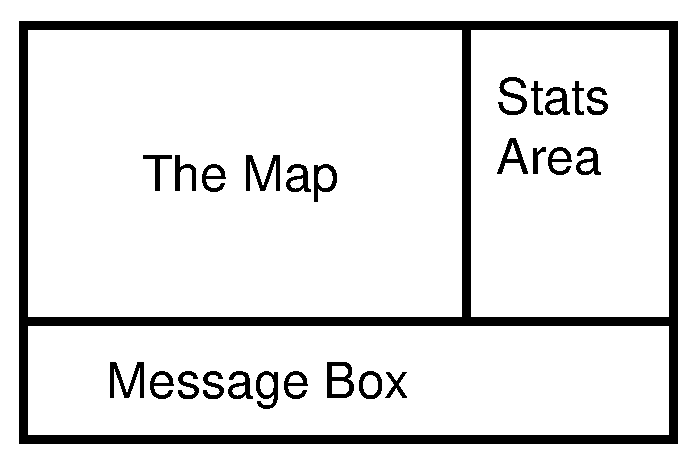
\includegraphics[scale=0.4]{screen}
\end{minipage}
\para\para

\sex{Exploring} \para

Try walking around, using either the numeric keypad (try numlock off and on) 
or the \key{hjklyubn} keys. To move in a given direction until you reach 
something interesting or see a hostile creature, press \key{Shift-direction}. 

If you want to know what a certain character on the screen represents, use the 
\key{x} (examine) command to get a short description. Climb staircases with
the \key{<} (up) and \key{>} (down) commands. Doors are opened simply by 
moving into them. Sometimes doors are hidden, and must be searched out by 
standing next to walls and resting (a number of commands do the same thing: 
\key{5} or \key{Shift-numpad-5} rest/search for a while, whereas \key{s} and 
\key{.} (period) do so for just a single turn).

The Dungeon gets more dangerous (but more interesting!) as you go down. If you 
get lost, you can access a map of the whole level you are on with the \key{X} 
command, which uses the whole screen. 

\para\para

\sex{Items} \para 

After walking around for a while, you will no doubt come across some items 
lying around (you may come across some monsters as well; for help in dealing 
with them skip to the Monsters section). This table lists the most basic item
types that appear and typical commands to use them:

\para

\begin{tabular}{cll}
\sex{Symbol} & \sex{Item type (typical commands)} & \sex{Comments} \\
\key{)}  & Weapons (\key{w}ield)                  & Move into monsters to attack them.\\
\key{(}  & Missiles (\key{f}ire)                  & Wield a bow to fire arrows. Press \key{f?} for help.\\ 
\key{[}  & Armour (\key{W}ear and \key{T}ake off) & Can be cursed, like weapons and jewellery. \\
\key{\%} & Food, corpses (\key{e}at and \key{c}hop up) & Dangerous chunks are coloured. \\
\key{\$} & Gold                                   & There are shops down below. \\
\key{?}  & Scrolls (\key{r}ead)                   & Scrolls mostly affect your environment.\\
\key{!}  & Potions (\key{q}uaff)                  & Potions affect you, in good or bad ways. \\
\key{=}  & Rings (\key{P}ut on and \key{R}emove)  & Rings can be helpful as well as malignant. \\
\key{"}  & Amulets (\key{P}ut on and \key{R}emove) & Amulets can be even subtler than rings. \\
\key{/}  & Wands (\key{Z}ap)                      & Identify these by zapping at monsters. \\
\key{+}  & Books (\key{r}ead, \key{M}emorise and \key{z}ap) & Press \key{z?} for information on spells.\\
\key{\char`\\} & Staves and rods (\key{w}ield and e\key{v}oke) \hspace{0.2em}
                                                  & Rods carry spells but they are very rare.
%\key{\}} & Miscellaneous items (e\key{v}oke)      & These will turn up only later. \\
\end{tabular}

\para

Some vital commands are given next. For a full list of commands, press \key{??}.
Don't be scared by the abundance of commands, you will only need a handful at 
the beginning. 

\para

\begin{minipage}[t]{7cm}
\sex{Most basic commands for new players} \\
\key{i} lists inventory \\
\key{d}	drops items \\
\key{g} or \key{,} pick up items from the ground \\
\key{gg} or \key{,,} for pickup menu \\
\key{x} examines a seen monster (has help on \key{?}) \\
\key{X} looks at the whole level (has help on \key{?}) \\
\key{>} goes deeper one level \\
\key{S} saves the game \\
\key{?} prints the help screen
\end{minipage}
%
\spacecolumn
%
\begin{minipage}[t]{7cm}
\sex{Somewhat advanced commands} \\
\key{p} prays (press \key{\^} for god information) \\
\key{Ctrl-P} shows previous messages \\
\key{Ctrl-F} searches for items dungeon-wide \\
\key{Ctrl-G} or \key{G} provides automated travel between levels \\
\key{o} provides automated exploration \\
\key{\#} dumps character to the file \texttt{name.txt} \\
\key{=} reassigns inventory or spell letters \\
\key{m} checks your current skills \\ 
\key{Ctrl-D} saves macros and key maps
\end{minipage}

\para

You will often want to get information on a particular item. If it is on the
ground, use the \key{x} command. If it is in your inventory, press \key{i},
followed by the item's slot key.

\para\para

\sex{Monsters} \para 

You will also run into monsters (most of which are represented by letters of 
the alphabet). You can attack a monster by trying to move into the square it 
is occupying. 
When you are wounded, you lose Health (displayed near the top of the stats 
list); these return gradually over time through the natural process of 
healing. If you lose all of your Health, you die. 
To survive, you will need to develop a few basic tactics: \\

\begin{minipage}{7cm}
\begin{abcliste}
\item[$\bullet$] 
   Never fight more than one monster at a time if you can help it. Back 
   into a corridor so that they fight you one-on-one. 
\item[$\bullet$] 
   If you are badly wounded, you can run away from monsters to buy some time. 
   Try losing them in corridors, or as a very last resort find a place where 
   you can run around in circles to heal while the monster chases you. 
\end{abcliste}
\end{minipage}
\spacecolumn
\begin{minipage}{7cm}
\begin{abcliste}
\item[$\bullet$] 
   Remember to use projectiles before engaging monsters in close combat. 
\item[$\bullet$] 
   Rest between encounters. Pressing \key{Shift-numpad-5} or \key{5} make
   you rest for a while (you will stop resting when fully healed). 
\item[$\bullet$] 
   Learn when to run away from things you can't handle --- this is important! 
   Often, it is wise to skip a dangerous level.
\end{abcliste}
\end{minipage}


\para\para

\sex{Death} \para 

Before long, you'll probably end up dead. 
Death in Crawl is permanent; you cannot just reload a saved game and start again
where you left off. The \key{S} (save) command exists only to let you leave a game 
part-way through and come back to it later.

\para

Well, that's it for the quick-start guide. This should help you through your 
first few games, but Crawl is extremely (some would say excessively) complex 
and cannot be adequately described in so short a document. So when you feel 
ready to start playing with magic, skills, and religions, browse the manual.

\para

Happy Crawling! 
\end{document}
